\chapter{Herramienta Web para Enseñanza e Investigación en Visión Artificial y Robótica}
En este capítulo se explica cómo se implementó la idea planteada paso a paso, detallando minuciosamente cómo se alcanzó cada uno de los hitos mencionados y aportando la explicación técnica de los problemas encontrados y las soluciones propuestas.

Se comenzará por describir el diseño de la aplicación robótica a través de la web en cuestión que simplificará el acceso de los usuarios al mundo de la robótica. Se especificarán los puntos desfavorables que desembocan en la necesidad de un mecanismo que resuelva, además de lo anterior, tanto los posibles defectos como la ubicación del peso del cómputo. Para el primer paso se especificará la arquitectura de cada uno de los módulos que componen el servidor remoto y su interfaz de abstracción, para luego desembocar en el diseño y arquitectura finales de la ``Ejecución Mixta'' que aportaran el mencionado cómputo en el cliente y la escalabilidad de la aplicación web.

\section{Servidor Web en Ejecución Remota}

\begin{figure}[!ht]  \centering\noindent
    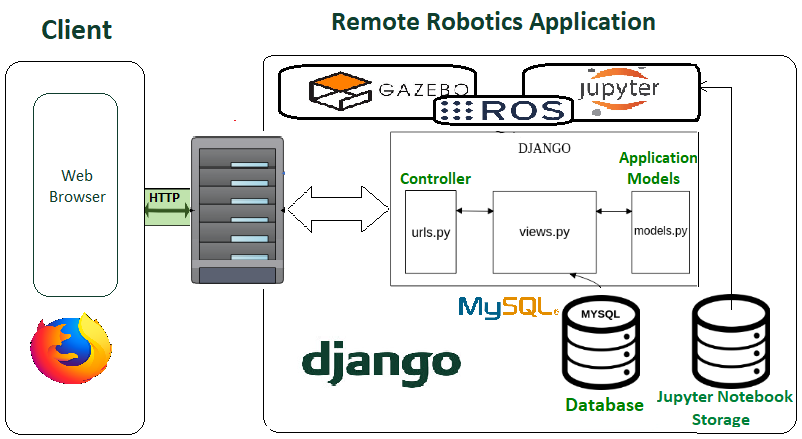
\includegraphics[width=1.20\textwidth,height=8cm]{figures/servidor_remoto_arquitectura.png}
    \caption{Arquitectura del Servidor en Ejecución Remota.}
    \label{remoteexecarch}
\end{figure}

Del mismo modo que no se puede comenzar la casa por el tejado, no podemos empezar con la implementación del mecanismo de la ``Ejecución Mixta'' sin una aplicación robótica a la que conectarla, lo que también servirá para sacar a la luz las carencias o puntos desfavorables relacionados con el servicio web aplicado a la robótica.

\subsection{Diseño del Servidor Web de la Aplicación}

El diseño del contenido prototípico que se quería servir a través de la aplicación web robótica utiliza Django como tecnología de servidor, Jupyter y Gazebo como herramientas en las que se basa la aplicación y sus versiones web para formar el interfaz de usuario y Apache como envoltura para entornos de producción. A fin de ilustrar el funcionamiento y la orientación de la herramienta, decidimos organizar el servicio como una aplicación para el aprendizaje de distintos ámbitos de la robótica por medio de ejercicios con contenido académico.

Como todo servicio web, estará ubicado en un punto físico que resultará siempre remoto al usuario que accede a él, es decir, que se ubica en una red distinta a la del usuario que accede a Internet. Por tanto, este servicio web se basará en el clásico entorno remoto en el que es el lado servidor el que carga con el peso computacional del servicio que ofrece, y el cliente accede a él de manera muy sencilla a través de los motores de búsqueda de su sistema.

Para el diseño de la funcionalidad hemos recurrido a los referentes en aplicaciones web de este tipo, concretamente a la plataforma JdeRobot-Academy, para partir de una organización inicial.

\subsection{Back-end del Servicio}

Como se puede ver en el esquema de arquitectura del servicio web (Fig. \ref{remoteexecarch}), se ha utilizado Django y su gran cantidad de librerías relacionadas con el servicio web y el acceso y gestión de bases de datos para Python para construir el \textit{back-end} o infraestructura del servidor remoto. Como parte de esta estructura de bajo nivel se diseñó una serie de plantillas HTML que actuarán como interfaz de usuario que están alimentadas por variables Python que provienen de las vistas o \textit{views} de Django, las cuales se encargan de la gestión y el procesado de todas las peticiones que los usuarios de la aplicación generan a través del interfaz. La parte más importante de las vistas es la transformación de las peticiones recibidas en este caso en ejercicios concretos de visión artificial y robótica. Para ello es necesario proveer al servidor con ficheros estáticos que harán las funciones de infraestructura de cada ejercicio, con el fin de actuar como capa de abstracción para que el usuario tenga un API sencillo de utilización del ejercicio y las herramientas utilizadas en el \textit{front-end} puedan transformar sus interacciones en acciones concretas sobre el ejercicio y sus agentes simulados o reales.

Cabe destacar que el servicio implementado cuenta con muchos módulos internos encargados de las herramientas básicas de usabilidad y experiencia de usuario, como el inicio de sesión y la gestión de sesiones activas, en las cuales no se va a profundizar al no ser objeto específico de este proyecto.

\begin{figure}[!hbtp]  \centering\noindent
    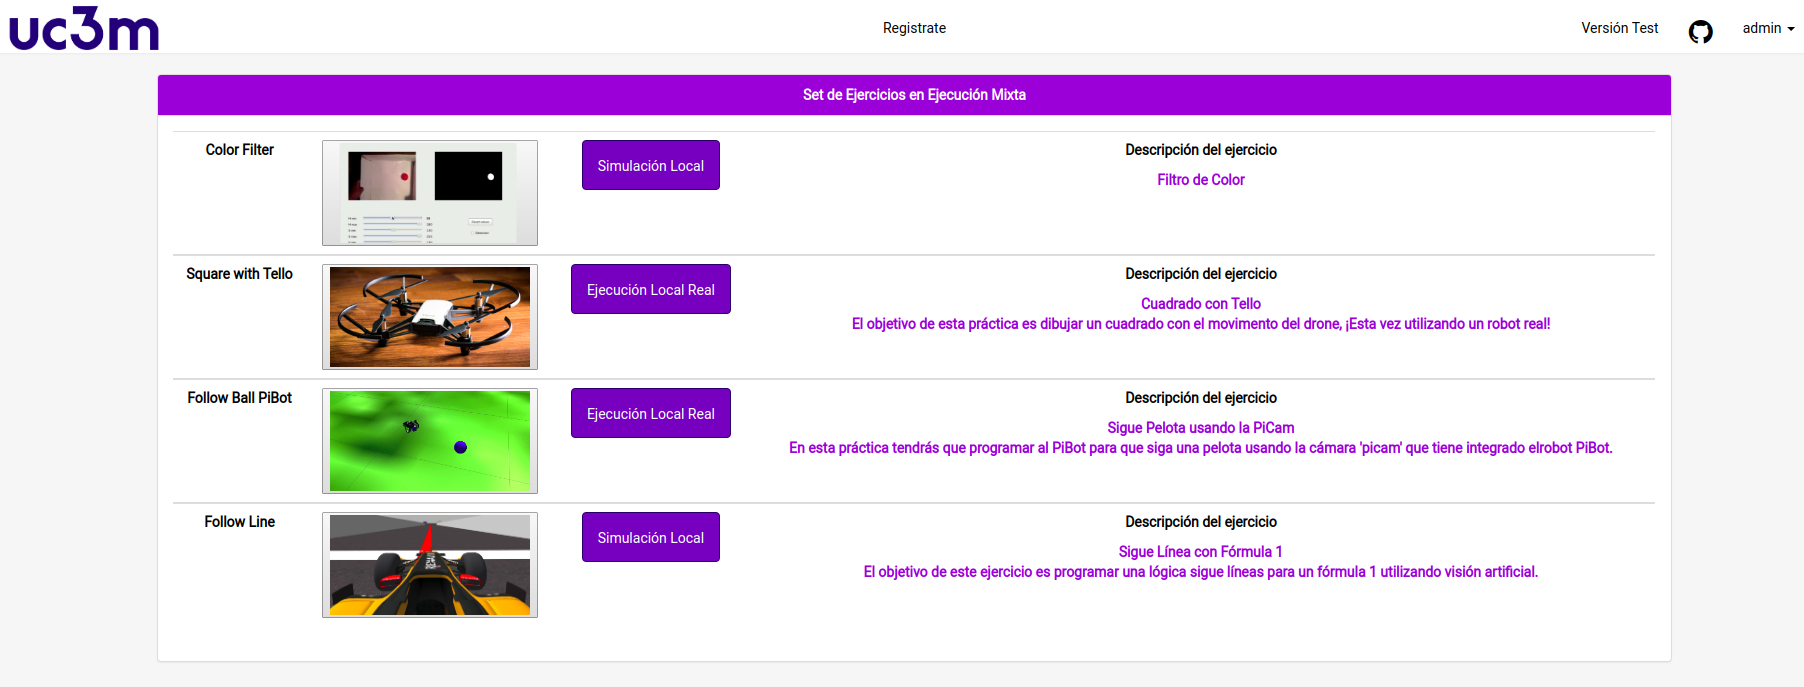
\includegraphics[width=0.99\textwidth]{figures/app_ui.png}
    \caption{UI de la Aplicación en Django}
    \label{appui}
\end{figure}

Como parte del \textit{back-end} encargado del soporte de servicio, se contará tanto con un servidor de Jupyter como con un servidor de Gazebo (\textit{gzserver}) que estarán en constante ejecución durante la solicitud y desarrollo de un ejercicio académico. 

Recordemos que Jupyter es una plataforma de escritorio (requiere instalación) con capacidad de visualización a través de la web. El motor computacional de Jupyter requiere del uso de un \textit{kernel} físico del equipo para llevar a cabo sus funciones, y luego comunica los resultados al interfaz web. Por tanto, el procesado de peticiones cuenta con señales de control que disparan el levantamiento de un servidor remoto de Jupyter (local al servidor web) que será el encargado de ejecutar el código del ejercicio del usuario.  Como se puede ver el contexto inicial es puramente local y supone asumir que el código a ejecutar para el ejercicio robótico proviene de la misma máquina que lo sirve, y por tanto se va a encargar de todo el cómputo. 

Por otro lado, la simulación a través de Gazebo sucede en un escenario análogo al de Jupyter, ya que también se trata de una aplicación de escritorio con interfaz web. Por tanto, también ha de levantarse un servidor de Gazebo que atienda a las peticiones de simulación. Todo lo anterior supone un grave problema atendiendo a la escalabilidad y la eficiencia computacional, dado que la conjunción de varios usuarios simultáneos generaría una carga de cómputo no asumible para el servicio, que para dar soporte a cada uno debería levantar una instancia de ambas aplicaciones.

En cuanto a la conexión entre ambas partes, simulador y código, utilizamos ROS como \textit{middleware} de comunicaciones dada su fácil integración con Gazebo y el lenguaje Python. Esto permite construir una aplicación completa y autocontenida asociada al código del ejercicio que creará el mecanismo de inter-comunicación a través de mensajes de ROS (\textit{ROS Messages}) que se intercambian por canales o \textit{topics} de publicación y suscripción de información (Listing. 4.1). De esta manera los resultados de las instrucciones que el usuario coloque en su código se reflejan en la simulación.

\begin{lstlisting}[language=bash, caption=Topics de ROS asociados a los Canales de Comunicación Internos]
~$ rostopic list
/F1ROS/cameraL/camera_info
/F1ROS/cameraL/image_raw
/F1ROS/cameraL/parameter_descriptions
/F1ROS/cameraL/parameter_updates
/F1ROS/cmd_vel
/F1ROS/odom
/clock
/gazebo/link_states
/gazebo/model_states
/gazebo/parameter_descriptions
/gazebo/parameter_updates
/gazebo/set_link_state
/gazebo/set_model_state
/rosout
/rosout_agg
/tf
\end{lstlisting}

De nuevo, todo este mecanismo añade demasiada carga al lado servidor, que empieza a requerir soporte computacional adicional para dar servicio, como granjas de ordenadores de soporte o procesadores adicionales. Además, cabe destacar también que el uso de un servicio web remoto como el descrito está muy limitado en cuanto a la variedad de robots soportados. Se ha de tener en cuenta que, por ejemplo en el uso de una cámara, el ejercicio que se construya estará supeditado al tipo de \textit{hardware} del que se disponga en el lado servidor, al entorno de servicio en el que la cámara será estática (lo que limita la riqueza de ejercicios que se pueden construir al estar siempre enfocando al mismo entorno), y en todo caso imposibilita el empleo de los robots de los que los usuarios puedan disponer.

Para poner este servicio en producción y que los usuarios puedan acceder a él es necesario el empaquetamiento de toda la estructura en una envoltura de servidor HTTP dado que Django no ofrece por sí mismo este soporte. La tecnología Apache interviene para cumplir esta función. Se trata simplemente de una capa de servidor HTTP orientado a dar un formato correcto a todas las peticiones generadas desde el servicio web y destinadas a él para que puedan viajar por Internet sin percances. Aporta también mecanismos extra de seguridad para proteger el servicio frente a las intrusiones y permite configurar una capa de TLS a través del protocolo SSL y el uso de certificados de encriptación de información.

Todo ello se refleja en los ficheros de configuración de servicio de Apache, compuestos por directivas que indican el tipo de cabeceras HTTP que deben llevar los mensajes, los \textit{endpoints} donde la aplicación web espera a recibir peticiones, la ubicación de los ficheros estáticos y la configuración básica de seguridad, permisos de actuación y servicio.

\subsection{Front-end de la Aplicación}

Una vez preparada la estructura básica de gestión de peticiones, se construye encima de la misma la capa de usuario o \textit{front-end} de la aplicación para los ejercicios. El agente encargado de disponer el interfaz de usuario será el navegador web del cliente. Este interfaz se basa en un cuadernillo de Jupyter que permita al usuario, desde el navegador, visualizar el resultado de una ejecución de código Python. Dado que los ejercicios emplearán algún tipo de robot o sensor, también se incluye en la interfaz una sección de simulación con GzWeb o divisiones auxiliares que contendrán la información necesaria para que el usuario pueda depurar y resolver el ejercicio, como visualizadores de imágenes de una cámara.

Así, la interacción del usuario se realiza sobre un \textit{Notebook} de Jupyter almacenado en el servidor cuya función es actuar como interfaz de edición de la aplicación (IDE), que enviará mensajes al \textit{kernel} del servidor para que compute.

\begin{figure}[!hbtp]  \centering\noindent
    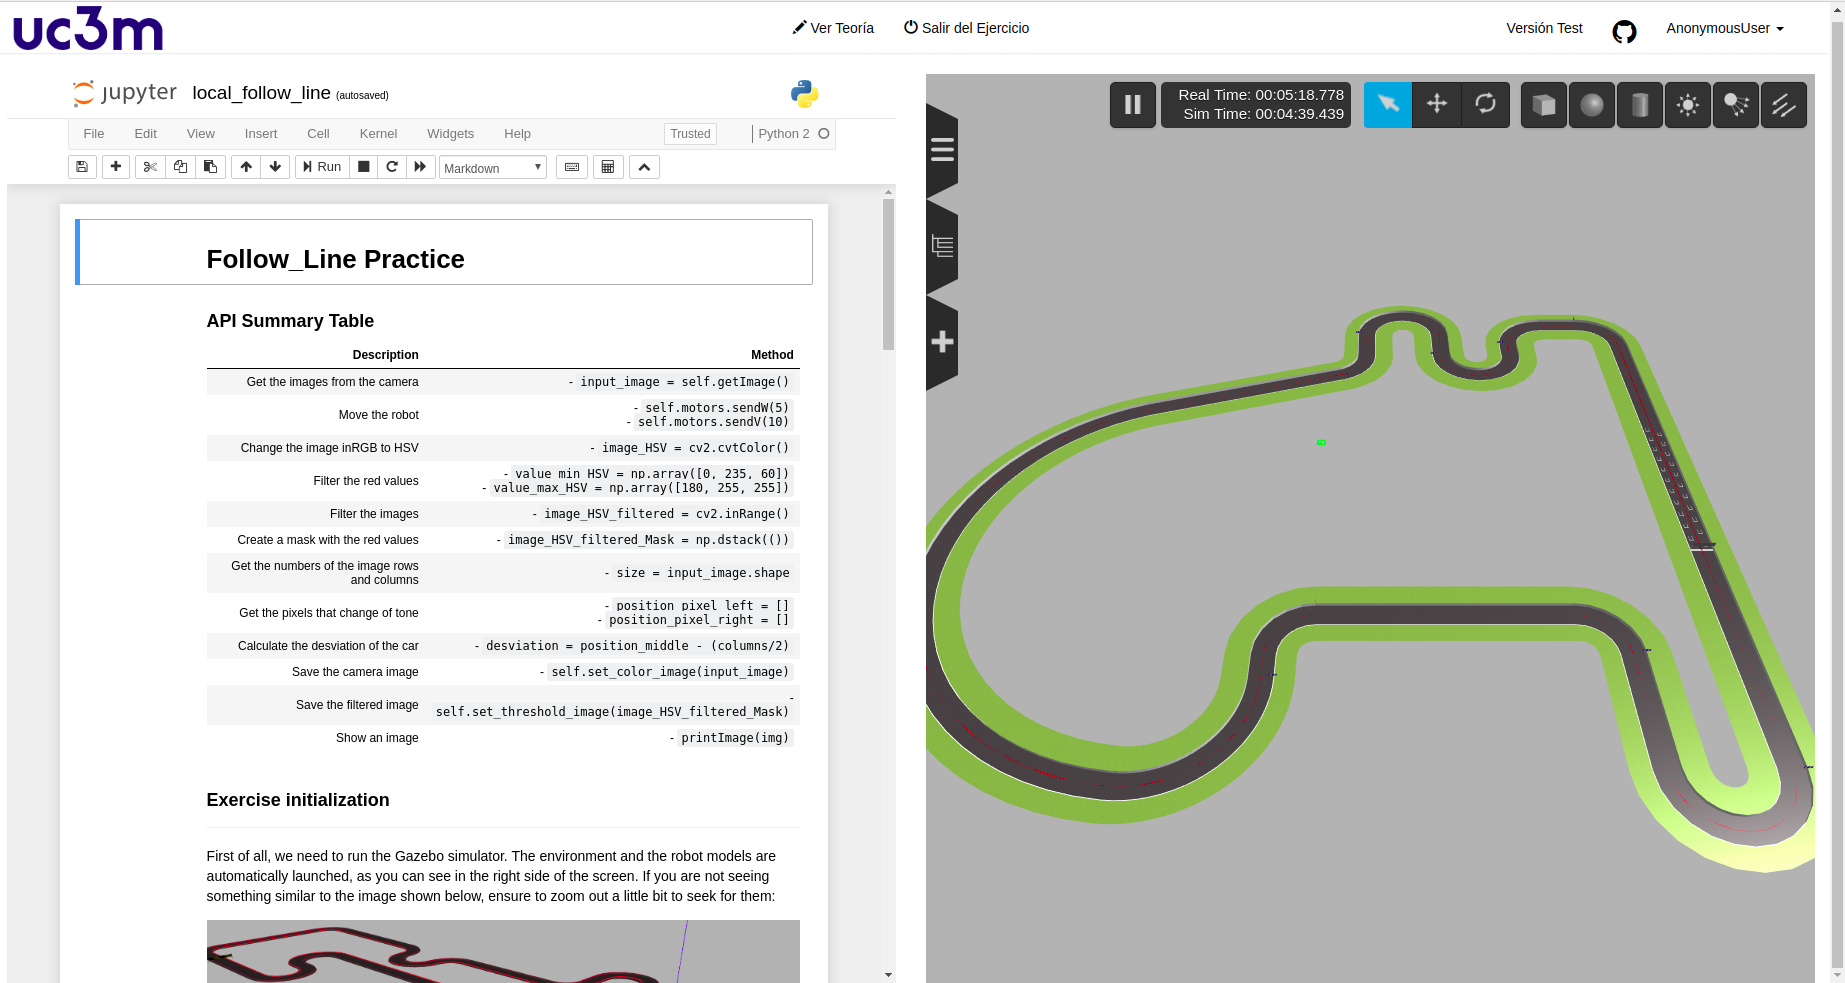
\includegraphics[width=0.99\textwidth]{figures/ui_simulation.png}
    \caption{UI de Simulación de la Aplicación}
    \label{simui}
\end{figure}

Se puede ver que el cliente web no asume ninguna carga de procesamiento, sino que sólo cuenta con un navegador que en todo momento solicita la visualización de varias aplicaciones que están corriendo coordinadas en el lado del servidor web.

\section{``Ejecución Mixta''}

\begin{figure}[!ht]  \centering\noindent
    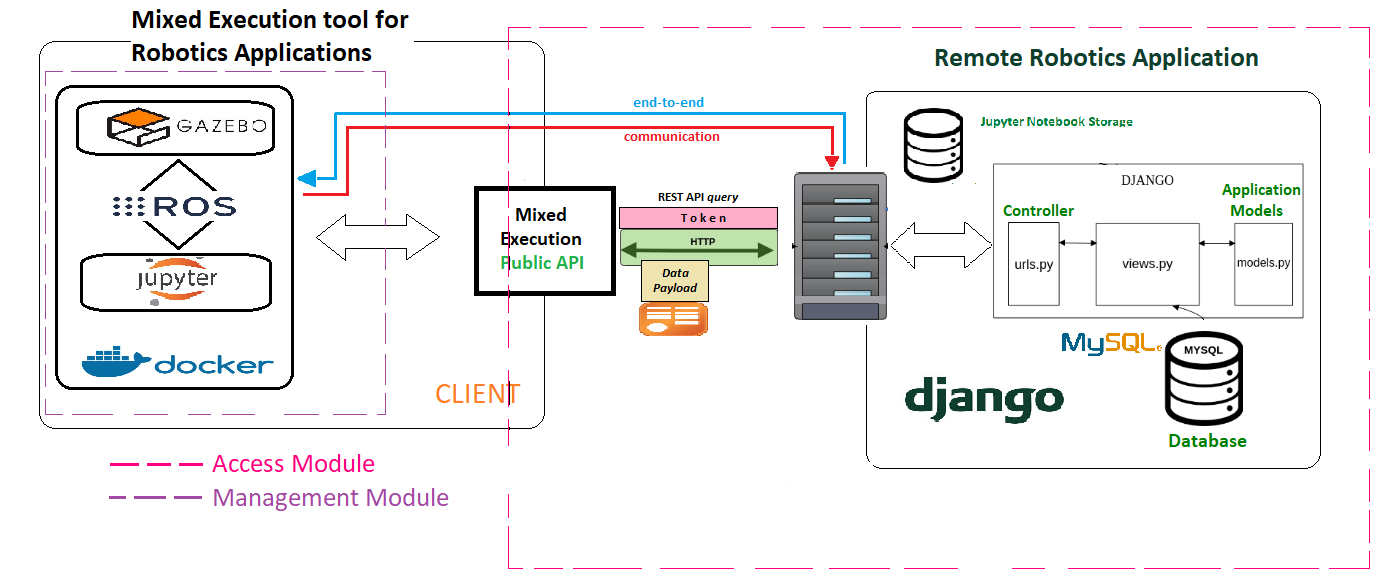
\includegraphics[width=1.20\textwidth,height=9cm]{figures/ejecucion-mixta-infograma.png}
    \caption{Arquitectura de la Ejecución Mixta para Aplicaciones de Robótica.}
    \label{mixedexecarch}
\end{figure}

En este punto, disponemos de una versión completamente remota del servicio de aprendizaje y docencia que se quiere construir. Se han relatado los problemas derivados de este tipo de servicio, y se puede ver claramente como no encajan con las características deseadas para la herramienta robótica objeto de esta tesis. Por tanto, y tras la investigación correspondiente, se procedió a la implementación de un \textit{local runtime}, es decir, de un entorno de ejecución utilizando un \textit{kernel} local al cliente, en comunicación constante con la aplicación web remota. Había que desarrollar un servidor remoto que contuviese la aplicación y el modelo de ejercicio creado y que, ante una nueva petición del ejercicio, estableciese una comunicación fluida con el \textit{kernel} del cliente para coordinar la ejecución en su \textit{hardware}, por medio del lanzamiento del servidor de ``Ejecución Mixta'' en su máquina. 

Partiendo del básico servidor web en Django (Fig. \ref{appstructure}), descrito anteriormente, con capacidad para atender a un cliente que solicitase un ejercicio por medio de un click en el interfaz web, se colocó la arquitectura de ``Ejecución Mixta'' debajo del botón sobre el que el usuario hace click para entrar al ejercicio que resolverá el mecanismo de enlazado y comunicación para disponer el entorno mixto.

Como se puede ver en la imagen (Fig. \ref{simui}) de la interfaz que ofrece el servidor web a su cliente, es necesario para el correcto funcionamiento de la herramienta que el receptor principal de los mensajes de ``Ejecución Mixta'' sea Jupyter, y por tanto también tiene sentido que se use como editor de código. Tras la conexión HTTPS con el servidor web, lo primero que debe hacer el cliente es especificar su dirección IP y el puerto en que está corriendo el servidor de Jupyter en su máquina dado que, como ya es sabido, es necesario que este escuche físicamente en una máquina para poder acceder al \textit{hardware} de la misma. De esta manera se puede establecer fácilmente un puente que permita que el servidor acceda a los datos generados por Jupyter desde un punto remoto, y los ofrezca al usuario como parte del interfaz, a través de un mecanismo de paso de mensajes de actualización periódicos. Esto requiere hacer unos cambios sobre el servidor provisto por el proyecto Jupyter con el fin de abrir el acceso a él desde el exterior, no sin antes establecer los correspondientes métodos de seguridad. Se profundizó en la arquitectura de servicio de Jupyter para poder adaptar su funcionamiento a nuestras necesidades.

Se infiere la necesidad de una especie de servidor en el lado cliente web que difunda la información de una ejecución local a quien la solicite. Este es precisamente el servidor de ``Ejecución Mixta''. Para lograr la ejecución del código del cliente localmente a través de órdenes generadas en el interfaz ofrecido por un servidor remoto, se hace indispensable proveer al servidor de ``Ejecución Mixta'', concretamente al \textit{kernel} de Jupyter, del código asociado al ejercicio para que pueda ejecutarlo, y también de un mecanismo de retorno de los resultados para que el servicio web pueda reflejarlos en el interfaz de visualización de usuario. Aquí comienza el mecanismo de establecimiento y supervisión de la conexión HTTPS que llevará a cabo la denominada Capa de Comunicación. La conexión con Jupyter puede hacerse de manera sencilla mediante el envío de un simple mensaje bajo el método OPTIONS, al que el servidor responderá con toda la información que necesitamos para el establecimiento de la conexión a través de cabeceras HTTP, entre ellas el \textit{token} de autenticación de Jupyter, los métodos y tipos de contenido que se aceptan, y el código CSRF\footnote{\href{https://www.geeksforgeeks.org/what-is-cross-site-request-forgery-csrf/}{What is CSRF and how to prevent it?}} necesario para enviar información al servidor de Jupyter desde otros puntos.

Al obtenerse esta información se ha de disponer un canal entre el servicio web remoto y el servicio de ejecución local, para lo cual no existen soluciones. Estudiamos el mecanismo de comunicación de la plataforma, que emplea principalmente el protocolo ZeroMQ\footnote{\url{https://zeromq.org/}} o 0MQ para el intercambio asíncrono de mensajes \textit{N-a-N} a través de la web. Esto nos proporciona, además de una plantilla para los tipos de mensajes que debemos enviar al \textit{kernel} de Jupyter, una idea bastante fiel del proceso que desencadena cada órden o petición que se le hace al servidor de Jupyter. También se utilizó \textit{sniffers}\footnote{\href{https://www.wireshark.org/\#1398253364-1-69}{Wireshark Sniffer}} para monitorizar el funcionamiento local de Jupyter (Fig. \ref{wireshark}). Este paso fue vital para comprender el procedimiento que debíamos seguir para iniciar una sesión de Jupyter completa y válida.

\begin{figure}[!hp]  \centering\noindent
    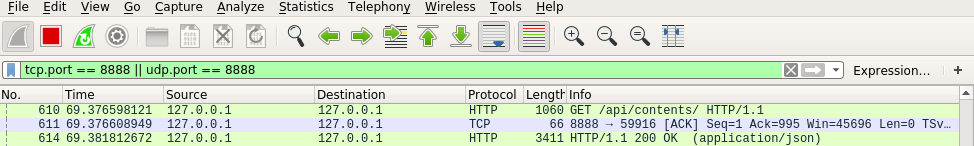
\includegraphics[width=0.99\textwidth]{figures/wireshark.png}
    \caption{Capura de Paquetes del Mecanismo de Comunicación de Jupyter}
    \label{wireshark}
\end{figure}

Por tanto tras el establecimiento, se puede comenzar con el intercambio de mensajes 0MQ. Aprovecharemos el REST API que ofrece Jupyter para la comunicación con el \textit{kernel} en tanto que este \textit{RESTfull Service}\footnote{\href{https://docs.oracle.com/javaee/6/tutorial/doc/gijqy.html}{What is a RESTfull Service?}} ofrece todo lo necesario para enviarle ficheros de código, órdenes de ejecución, órdenes de control (reinicio, apagado, encendido, pausa, cambio de lenguaje, limpieza de salidas, etc.) (Fig. \ref{jupyter_rest_api}) y, en general, lo necesario para facilitar el uso de la plataforma a través de la web. Por tanto, por el canal de ``Ejecución Mixta'' estaríamos enviando, principalmente, mensajes HTTP sobre una capa de TLS con datos de tipo 0MQ en el cuerpo, destinados a Jupyter que viajan por Internet.

\begin{figure}[!ht]  \centering\noindent
    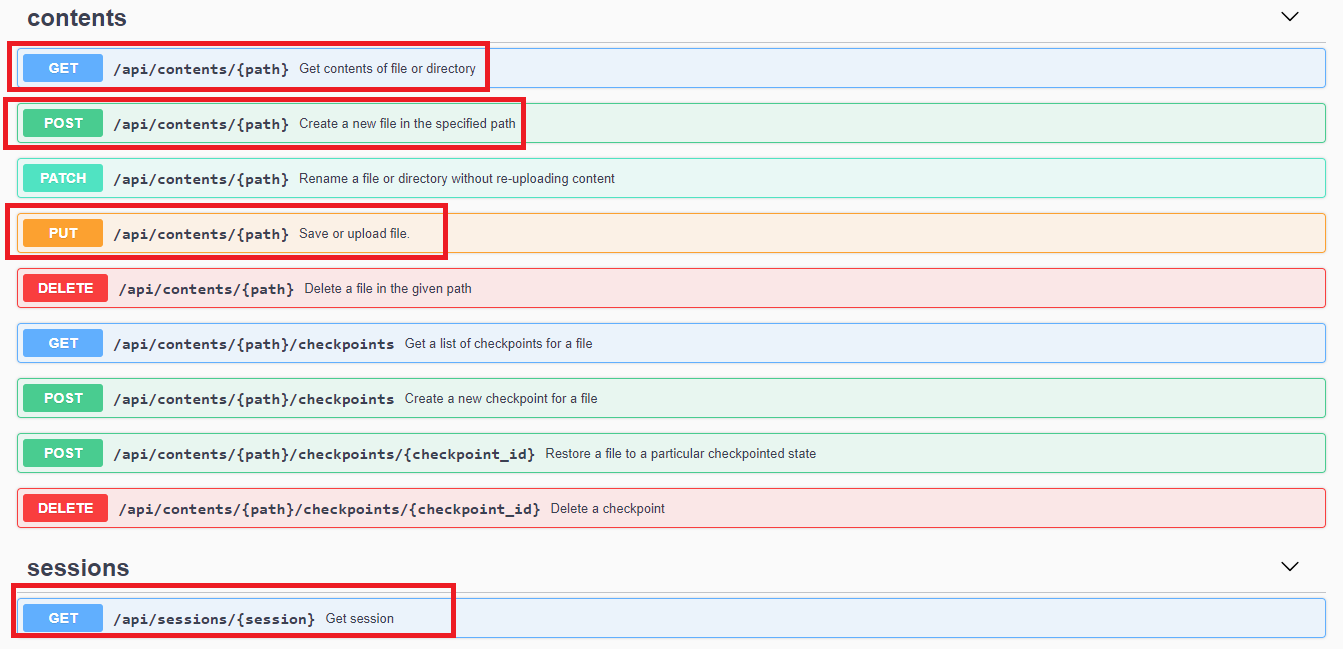
\includegraphics[width=0.99\textwidth]{figures/jupyter_rest_api.png}
    \caption{REST API de Jupyter}
    \label{jupyter_rest_api}
\end{figure}

En base al conocimiento obtenido del motor de comunicación de Jupyter, seleccionamos aquellos métodos del REST API que necesitaríamos, marcados en la imagen superior. Se muestra a continuación un ejemplo del mensaje que se enviaría al servidor de Jupyter para hacer llegar el código al \textit{kernel} encargado de un cuadernillo concreto:

\lstset{
   language=JavaScript,
   backgroundcolor=\color{lightgray},
   extendedchars=true,
   basicstyle=\footnotesize\ttfamily,
   showstringspaces=false,
   showspaces=false,
   numbers=left,
   numberstyle=\footnotesize,
   numbersep=9pt,
   tabsize=2,
   breaklines=true,
   showtabs=false,
   captionpos=b
}
\begin{minipage}{\linewidth}
\begin{lstlisting}[caption=Formato de Mensajes de ``Ejecución Mixta'']
const url = 'http://'+_ip+':'+_port+'/api/contents/' + nbname;
const data_put = ' {"type": "notebook",
                    "format": "json",
                    "content": ' + nbcontent + '} ';
const message = {
        headers:{'Content-Type':'application/json',
                 //'Authorization': 'token ' + _token,
                },
        body:data_put,
        method:"PUT"
};
\end{lstlisting}
\end{minipage}

donde cada variable que aparece en el mensaje (\textit{\_ip, \_port, nbname,\_token, nbcontent}) sería establecida por el servidor web y contendría la dirección del servidor Jupyter y el contenido y nombre del cuadernillo que queremos enviar, almacenado en el servidor remoto y solicitado por el usuario web. El formato de todos los mensajes es similar, en tanto que se trata de peticiones HTTP como se puede ver en la constante \textit{message} con el formato de cuerpo 0MQ que se refleja en la constante \textit{data\_put}. Este tipo de mensajes, con su respectiva codificación, constituye el tipo de mensajes a intercambiar por la herramienta ``Ejecución Mixta'' para el establecimiento y envío iniciales.

El proceso de comunicación con Jupyter comenzaría por el establecimiento de la conexión, donde se crea una sesión de ejecución, continuaría con el envío del código del cuadernillo y de cada fichero de código de aplicación auxiliar que necesite el ejercicio, para acabar con una orden de inicio del \textit{kernel} del lenguaje adecuado encargado de la ejecución, que se montará sobre un núcleo latente en el sistema del cliente web. La utilización de direcciones IP públicas, el protocolo HTTP (estándar de Internet) que utiliza por defecto el puerto 8080 (puerto de Internet, abierto a mensajes transportados sobre TCP o UDP por la red, con cualquier origen) que puede atravesar \textit{firewalls} y resolver conexiones sea cual sea el dominio público, y el \textit{token} de autorización embebido en los mensajes garantizan la conectividad y la integridad de la sesión de Jupyter, así cómo el funcionamiento entre sistemas bajo distintas redes o sub-redes de la misma red.

En este punto del desarrollo, hemos superado el principal obstáculo de la ``Ejecución Mixta'' e implementado un mecanismo capaz de ejecutar código entre redes, con actualización de los resultados en tiempo real en ambos lados servidor  y cliente web. Se completa así el primer ciclo de trabajo, no sin antes realizar los tests convenientes de funcionamiento y desempeño y el análisis de los resultados. La herramienta ya es capaz de conectar un código remoto (aplicación robótica) con un ``robot'' local (cámara). Esto sortea tanto el obstáculo de desbordamiento de cómputo en el lado servidor, pues es ahora el cliente el que carga con la mayor parte del peso computacional, como la limitación de \textit{hardware} conectable a la aplicación web, ya que ahora el cliente puede emplear su propia cámara o incluso sus propios robots en los ejercicios, accesibles desde su máquina y su red, pero no desde el exterior.

Sin embargo, la dependencia de este servidor de ejecución local supone para el cliente la instalación de todas las herramientas, tanto Jupyter como Gazebo y ROS, para mantener el soporte del servicio web de manera local. Las ventajas obtenidas se ven empañadas por una serie de desventajas claras entre las que se encuentran principalmente el proceso de instalación (tedioso, requiere espacio de disco del cliente) y la compleja organización inter-plataforma necesaria para comunicar las herramientas locales. El usuario necesitaría un programa encargado de cumplir estas funciones, lo cual desmontaría el servicio web.

La alternativa diseñada pasa por utilizar contenedores Docker (lo cual cambiará sustancialmente el mecanismo de comunicación), sobre los que se puede construir una arquitectura de módulos que cuente con un mecanismo interno de comunicación entre plataformas y otro externo que se comunique con la aplicación remota. Por medio de Docker se puede conservar la funcionalidad previa, evitar el proceso de instalación y organizar de alguna manera la comunicación entre un agente remoto y los servicios locales al cliente de la ``Ejecución Mixta''.

Hubo que estudiar el motor de Docker y su funcionamiento para crear un \textit{DockerFile} con instrucciones en lenguaje SHELL para virtualizar una distribución Ubuntu con todas las herramientas y aplicaciones auxiliares involucradas en la ``Ejecución Mixta'', para que utilizar la herramienta resultase tan fácil como descargar la imagen Docker y levantar el contenedor. Utilizar un contenedor Docker para empaquetar los procesos necesarios e incluir seguridad supone añadir complejidad el mecanismo de comunicación, en tanto que Docker levanta su propia sub-red dentro de la red del cliente, lo que nos deja una intratable sub-red dentro de una red distinta desde el punto de vista del servidor web. Se replanteó el mecanismo de comunicación para que utilizase el navegador del cliente web como intermediario entre el usuario y la aplicación robótica en lugar de la previa comunicación punto a punto, el cual sí que tiene conectividad directa con una sub-red de su propia red. Por tanto, el servidor web abre ahora una comunicación con el \textit{browser} del cliente en lugar de directamente con el servidor Jupyter, y éste actúa como \textit{proxy} reenviando cada mensaje donde corresponde a través de una secuenciación programada en código JavaScript, de manera que tanto de cara al cliente como al servidor web, la comunicación sigue siendo la misma que en el paso anterior, esta vez con un origen o destinatario distinto. Simplemente se trata de añadir la lógica del \textit{proxy} para que viaje con la aplicación que se sirve al usuario web. El navegador ya utiliza protocolos como STUN o ICE que permiten descubrir e interaccionar con ambas partes del mecanismo. Así, los mensajes reenviados por el navegador serán recibidos por un módulo secuenciador de ``Ejecución Mixta'', que procesará la información que llega para orquestar el correcto inicio del entorno y los agentes, traduciendo las órdenes JavaScript iniciales a comandos de lanzamiento (Listing. 4.3) y entregando las órdenes de ejecución a quien corresponda (Listing. 4.4).

\begin{lstlisting}[language=bash, caption=Código de Inicio del Secuenciador]
#!/bin/bash

rm -rf /tmp/.X0-lock

Xvfb -shmem -screen 0 1280x1024x24 &

source /opt/jderobot/setup.bash
source /opt/ros/kinetic/setup.bash
source /opt/jderobot/share/jderobot/gazebo/gazebo-assets-setup.sh
export PYTHONPATH=$PYTHONPATH:/home/jderobot/.exercises

cd ~/gzweb
npm start &

cd ~/volume/user/exercise

jupyter nbextension enable hide_input/main --user
jupyter nbextension enable init_cell/main --user
jupyter notebook --ip=0.0.0.0 --allow-root &

cd ~

EXTENSION=`echo "$1" | cut -d'.' -f2`
if [ $EXTENSION = "world" ]
  then
    roscore &
fi

if ! [ -z "$2" ]
  then
    python ~/referees/$2 &
fi

if ! [ -z "$1" ]
  then
    EXTENSION=`echo "$1" | cut -d'.' -f2`
    if [ $EXTENSION = "launch" ]
      then
        roslaunch /opt/jderobot/share/jderobot/gazebo/launch/$1
    else
        rosrun gazebo_ros gazebo /opt/jderobot/share/jderobot/gazebo/worlds/$1
    fi
else
    tail -f /dev/null
fi
\end{lstlisting}
\begin{lstlisting}[language=bash, caption=Reenvío de Mensajes]
[I 11:51:09.187 NotebookApp] Saving file at /thumbnail_follow_line.png
[Gazebo] Sat Jan 11 2020 11:51:09 GMT+0000 (Coordinated Universal Time) Received Message: {"op":"advertise","id":"advertise:~/heartbeat:14","type":"heartbeat","topic":"~/heartbeat"} from http://127.0.0.1:8080 ::ffff:172.17.0.1
[Python Process] Sat Jan 11 2020 11:51:09 GMT+0000 (Coordinated Universal Time) Received Message: {"op":"publish","id":"publish:~/heartbeat:15","topic":"~/heartbeat","msg":{"alive":1}} from http://127.0.0.1:8080 ::ffff:172.17.0.1
[I 11:51:11.758 NotebookApp] 302 GET /notebooks/world.png (172.17.0.1) 0.95ms
[I 11:51:11.847 NotebookApp] Adapting to protocol v5.1 for kernel 368a1e46-acc2-4976-acf3-25528ae77d77
\end{lstlisting}

El API de inicio de la ``Ejecución Mixta'' fue enriquecido con la aparición de los parámetros característicos de Docker que permiten crear un puente seguro entre un elemento virtualizado y su homólogo en la máquina anfitrión. Un ejemplo de esto es el mecanismo de acceso a la cámara integrada en el sistema cliente desde el interior de un contenedor Docker, resuelto con el mapeo \textit{-v /dev/video0:/dev/video0}, o la redirección de interfaces de escucha del sistema a sus correspondientes dentro del contenedor (\textit{-p 8888:8888 -p 8889:8889 -p 8080:8080}).

El contenedor de ``Ejecución Mixta'' ejecuta tanto la lógica como la simulación y aplicaciones auxiliares como \textit{plugins} o \textit{drivers} robóticos que actúen como controlador del dispositivo \textit{hardware} real. El mecanismo interno de comunicaciones a través de ROS pasa ahora por el secuenciador del denominado Módulo de Gestión, configurado para actuar de intermediario (Listing. 4.5), que reenvia los mensajes a quien corresponde y elabora una respuesta destinada al servicio web remoto a través de un canal WebSockets, envuelto con una capa HTTPS para que éste último lo procese (Fig. \ref{mixedexecarch}).
\begin{minted}[
    gobble=4,
    frame=single,
    linenos
  ]{yaml}
    Camera:                               # follow_line.yml
      Topic: "/F1ROS/cameraL/image_raw" 
      Name: follow_line_camera
    Motors:
      Topic: "/F1ROS/cmd_vel"
      Name: follow_line_motors
      MaxV: 40
      MaxW: 2
    Websockets:
      Host: 0.0.0.0 
      Port: 9002
      SSL: False
      Cert: '/etc/certs/fullchain1.pem' 
      Key: '/etc/certs/privkey1.pem'
\end{minted}
\begin{lstlisting}[caption=Configuración de Canales Inernos del Secuenciador en formato YAML]
\end{lstlisting}

La inclusión de la ``Ejecución Mixta'' ya no supone ninguna carga de cómputo para el lado servidor de la aplicación web y queda eliminado el proceso de instalación, dado que todas las dependencias están agrupadas en el contenedor. Lanzar la ``Ejecución Mixta'' pasa ahora por utilizar el API de Docker de control de contenedores, que pondrá en marcha todos los sub-sistemas necesarios para el funcionamiento de la aplicación robótica y los dejará disponibles para su consulta desde el exterior, por parte del servidor remoto a través del secuenciador o \textit{proxy} web. Así, la aplicación puede enviar cualquier tipo de orden de ejecución en formato Python al servidor de Jupyter, que materializará esa orden en el simulador Gazebo a través de los canales ROS o, incluso, en el robot o sensor real conectado al sistema del cliente. La aplicación robótica le indicará al secuenciador qué sub-procesos necesita para el funcionamiento de un ejercicio robótico concreto.

Para implementar el soporte de simulación, se diseñó un sistema de configuración que permite indicar los elementos, robots y características que debe tener la escena simulada a través de Gazebo (Fig. \ref{gzworld}), haciendo uso de ficheros de extensión \textit{.world} o \textit{.launch}, siendo los primeros un subconjunto del lenguaje de marcado XML que indica los agentes involucrados en la simulación (Listing. 4.7), y el segundo un configurador inteligente que permite lanzar, además del mundo de simulación, una serie de nodos que se puedan necesitar para controlar por ejemplo las interfaces de un determinado robot (Listing. 4.6). 

\begin{figure}[!hbtp]  \centering\noindent
    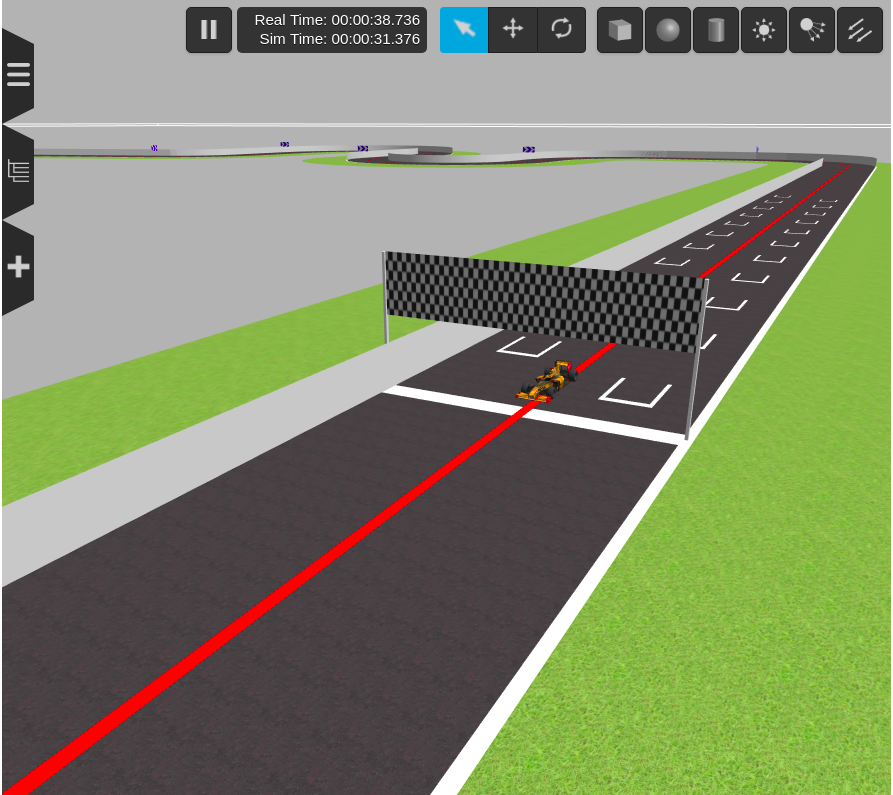
\includegraphics[width=0.9\textwidth]{figures/world_gazebo.png}
    \caption{Escenario de Simulación}
    \label{gzworld}
\end{figure}

\begin{lstlisting}[language=XML, caption=Configuración de Lanzamiento de Simulaciones]
<?xml version="1.0" encoding="UTF-8"?>
<launch>
  <!-- We resume the logic in empty_world.launch, changing only the name of the world to be launched -->
  <include file="$(find gazebo_ros)/launch/empty_world.launch">
    <arg name="world_name" value="f1_1_simplecircuit.world"/> <!-- Note: the world_name is with respect to GAZEBO_RESOURCE_PATH environmental variable -->
    <arg name="paused" value="false"/>
    <arg name="use_sim_time" value="true"/>
    <arg name="gui" value="true"/>
    <arg name="headless" value="false"/>
    <arg name="debug" value="false"/>
    <arg name="verbose" default="false"/>
  </include>  
</launch>
\end{lstlisting}

\begin{lstlisting}[language=XML, caption=Configuración de Lanzamiento de Simulaciones]
<?xml version="1.0" ?>
<sdf version="1.5">
  <world name="default">
    <scene>
      <grid>false</grid>
    </scene>
    <!-- A global light source -->
    <include>
      <uri>model://sun</uri>
    </include>
    <include>
	    <uri>model://pista_simple</uri>
	    <pose>0 0 0 0 0 0</pose>
    </include>
    <include>
      <uri>model://f1_renault</uri>
      <pose>53.462 -10.734 0.004 0 0 -1.57</pose>
    </include>
    <scene>
        <sky>
            <clouds>
                <speed>12</speed>
            </clouds>
        </sky>
     </scene>
  </world>
</sdf>
\end{lstlisting}

Con ello, al lanzar la herramienta se indicará qué fichero de configuración se quiere usar a través de instrucciones del API de ``Ejecución Mixta'', que se ocupará de levantar tanto la simulación como la red de comunicación interna basada en ROS como se puede ver en el \textit{snippet} de código inferior (Listing. 4.8), y la capa de abstracción que permite al usuario programar su robot y acceder a toda la funcionalidad mientras se materializan los cambios en el simulador.

\begin{minted}[
    gobble=4,
    frame=single,
    linenos
  ]{python}
    class ListenerCamera:
        def __init__(self, topic):
            
            self.topic = topic
            self.data = Image()
    
        # [...]
    
        def start (self):
     
            self.sub = rospy.Subscriber(self.topic, ImageROS,
                                        self.__callback)
    
    class PublisherMotors:
     
        def __init__(self, topic, maxV, maxW):
    
            self.maxW = maxW
            self.maxV = maxV
    
            self.topic = topic
            self.data = CMDVel()
            self.pub = rospy.Publisher(self.topic,
                                       Twist,
                                       queue_size=1)
            rospy.init_node("FollowLineF1")
    
        # [...]
    
        def publish (self):
    
            self.lock.acquire()
            tw = cmdvel2Twist(self.data)
            self.lock.release()
            self.pub.publish(tw)
    
    class FollowLine():
        
        def __init__(self):
            cfg = readConfig()
    
            cameraTopic = cfg["Camera"]["Topic"]
            motorsTopic = cfg["Motors"]["Topic"]
            maxv = cfg["Motors"]["MaxV"]
            maxw = cfg["Motors"]["MaxW"]
    
            self.camera = ListenerCamera(cameraTopic)
            self.motors = PublisherMotors(motorsTopic, maxv,
                                          maxw)
    
            # [...]
\end{minted}
\begin{lstlisting}[caption=Creación de la Red Interna de Comunicación]
\end{lstlisting}

Dada la filosofía modular interconectada que se había diseñado hasta este momento, el enfoque para el caso de querer controlar un robot real desde el lado cliente pasaba sencillamente por crear su controlador, e incluirlo como aplicación auxiliar lanzada dentro de la herramienta y orquestada como un módulo más por el secuenciador.

Se tiene una herramienta que actúa como \textit{middleware} entre un servicio web remoto y una serie de aplicaciones locales al cliente capaz de lanzar un proceso de ejecución compartida con una serie de ventajas claras, entre las que se encuentran el uso de robots reales del cliente, el bajo cómputo en el lado servidor web, la versatilidad de contenidos que se puede crear para la aplicación y, sobre todo, la accesibilidad a las aplicaciones robóticas.

\subsection{Diseño e Infraestructura de la herramienta}

En esta sección abordaremos el diseño final de las distintas capas que componen la herramienta y la jerarquía establecida. Se puede ver en el infograma (Fig. \ref{mixedexecarch}) que la solución ideada para la ``Ejecución Mixta'' se divide claramente en dos módulos, cada uno sub-dividido a su vez en una serie de capas encargadas de una parte específica del proceso:

\begin{itemize}
    \item [\textbullet] El primero de ellos es el \textbf{módulo de acceso}. Este módulo será el encargado de dirigir la comunicación entre el lado servidor y el lado cliente de la aplicación para que se produzca la ``Ejecución Mixta''. Organizará ambas partes y actuará como un secuenciador que decidirá en cada momento quién lleva el peso de la comunicación. Su propósito principal será el de garantizar el acceso a la herramienta.
    \item [\textbullet] El otro es el \textbf{módulo de gestión}. Estará recubierto por un API público que permitirá a las aplicaciones web externas realizar la conexión y aprovechar las funciones de ``Ejecución Mixta'' para ofrecer un servicio. Será el encargado de redirigir cada petición y respuesta de la aplicación al proceso que corresponda de forma segura, dentro de la ejecución del cliente.
\end{itemize}

Dada la clara distinción entre las distintas sub-tareas que realiza cada módulo, consideramos adecuado bajar otro escalón en cuanto a la arquitectura, y dividir cada módulo en capas encargadas de tareas sencillas, sobre las que se pudiese construir de manera modular. 

\subsubsection{Capa de Aplicación}

\begin{figure}[!hbtp]  \centering\noindent
    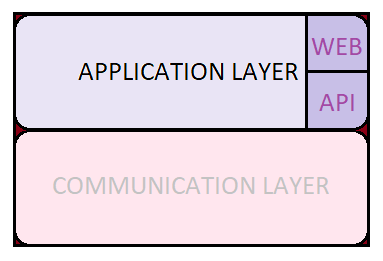
\includegraphics[width=0.6\textwidth]{figures/layer4.png}
    \caption{Módulo de Acceso: Capa de Aplicación}
    \label{layer4}
\end{figure}

La capa de aplicación tendrá la tarea específica de emparejar la funcionalidad que ofrece la aplicación remota como servicio con la información que necesita de la ejecución en el lado cliente para dar soporte a dicha funcionalidad. Requerirá de la intervención de dos agentes para cumplir su tarea:

\begin{itemize}
    \item [--] Será necesario que la aplicación robótica que se ofrece a través de la web que quiere beneficiarse de la ``Ejecución Mixta'' inicie la conexión con el cliente remoto, en calidad de cliente de ``Ejecución Mixta''. Esto es así dada la naturaleza de la información a la que más tarde pedirá acceso, la cual se genera completamente en el cliente durante la ejecución y pondrá a disposición de quien la solicite. El cliente de la aplicación web hace las funciones de servidor de la herramienta, ya que está pensada para ser colocada en el lado del cliente web.
    \item [--] Con la conexión iniciada, esta capa debe solicitar la información que necesite al servidor de ``Ejecución Mixta'', en tiempo de ejecución, para que la aplicación funcione como se espera. Esta solicitud se realizará a través del API de ``Ejecución Mixta''.
\end{itemize}

Así, el mecanismo completo de la capa de aplicación comenzará por establecer la conexión con la herramienta, utilizando uno o varios \textit{endpoints} en función de los canales de comunicación que se quiera establecer para recopilar la información necesaria y generará un comando específico para configurar en la herramienta el tipo de enlace que se requiere y el conjunto de herramientas que se necesita para la ejecución.

\begin{lstlisting}[language=bash, caption=Comando de configuración de Ejecución Mixta]

mkdir -p /tmp/siguelineaIR/ && docker run --rm -e DISPLAY=:0
-e JDEROBOT_SIMULATION_TYPE=REMOTE --entrypoint 
/entrypoint_mixed_execution.sh -v 
/tmp/siguelineaIR:/home/jderobot/volume/user/exercise:rw 
-p 8888:8888 -p 8080:8080 -p 9001:9001 -p 9002:9002 
-it tfmdocker/local:dev f1_1_simplecircuit.launch

\end{lstlisting}

\subsubsection{Capa de Comunicación}

\begin{figure}[!hbtp]  \centering\noindent
    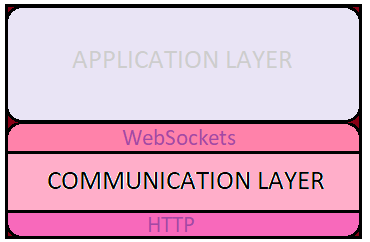
\includegraphics[width=0.6\textwidth]{figures/layer3.png}
    \caption{Módulo de Acceso: Capa de Comunicación}
    \label{layer3}
\end{figure}

Encargada del establecimiento de los canales de comunicación entre la aplicación robótica externa y la herramienta de ``Ejecución Mixta'' una vez iniciada la conexión. Se utilizará principalmente el protocolo HTTP para la comunicación que tiene lugar a través de Internet y que pretende conectar la herramienta y la capa de aplicación. El formato de los mensajes intercambiados será similar al de un REST API basado en solicitudes y respuestas HTTP utilizando los métodos clásicos: GET, POST, PUT, DELETE y OPTIONS.

Adicionalmente se utilizará un medio WebSockets para el intercambio de mensajes ligeros, más relacionados con el interfaz de usuario de la aplicación y aquella información que requiere un refresco de carga ligera pero constante. Se utilizará también como canal auxiliar para la información que necesiten enviar los agentes y procesos en ejecución durante la ``Ejecución Mixta'', en caso de necesitarse.

\subsubsection{Capa de Seguridad}

\begin{figure}[!hbtp]  \centering\noindent
    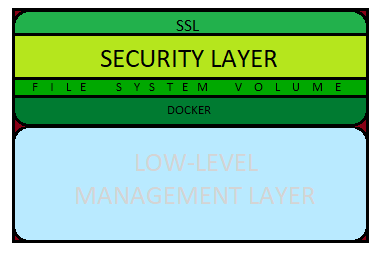
\includegraphics[width=0.6\textwidth]{figures/layer2.png}
    \caption{Módulo de Gestión: Capa de Seguridad}
    \label{layer2}
\end{figure}

Debemos distinguir dos niveles de seguridad en el proceso de ``Ejecución Mixta'':

\begin{itemize}
    \item [--] En primer lugar, hay que garantizar la fiabilidad e integridad de los mensajes intercambiados con la herramienta. Al ser tanto HTTP como WebSockets dos protocolos en los que la información viaja en claro, como texto plano, por el canal de comunicación, decidimos incluir una capa que garantiza seguridad a través del protocolo SSL, que también asegurará que los mensajes no se corrompan. Este nivel tiene un grado bajo de criticidad.
    \item [--] Por otro lado, existe un alto riesgo cuando se trata de permitir que un código cuya fuente es externa se ejecute en nuestro sistema. Esto es precisamente lo que se pretende hacer con esta herramienta, de manera que se debe asegurar que, sea cual sea la fuente del código y su contenido, los problemas de seguridad se pueden contener, evitando que actúen sobre el sistema del cliente, el cual lleva a cabo la ejecución. Esta es una de las funciones del contenedor Docker.
\end{itemize}

Para mantener segura la conexión entre cliente y servidor de ``Ejecución Mixta'' y entre cliente y servidor web a través de Internet utilizamos el protocolo TLS a Nivel de Transporte según la clasificación OSI, que asigna una serie de certificados SSL basados en criptografía asimétrica a cada agente de la comunicación para ser autenticados a la hora de intercambiarse la clave simétrica con la cual se pueden decodificar los datos intercambiados, que viajan encriptados en todo momento. Así funcionan la mayoría de sitios web en la actualidad.

El mayor peso en cuanto a seguridad recae sobre la tarea para la que ha sido diseñada la herramienta. El código que proviene del servidor web puede no ser de confianza o de dudosas intenciones, por lo que no se puede permitir a la ligera su ejecución en la máquina del cliente, dado que esto podría conllevar graves riesgos de pérdida de datos (mediante instrucciones de borrado de disco que viajasen en el código), malfuncionamientos y ataques de toda clase. Por ello, se ha montado lo que se denomina ``volumen'' (Fig. \ref{volumen}) sobre el sistema de ficheros local del servidor de ``Ejecución Mixta'' (cliente web), y se ha restringido el acceso del contenedor Docker y de las instrucciones que en él se ejecutan a este volumen, impidiendo en todo caso que cualquier suceso tenga consecuencias o repercusiones fuera de él. 

\begin{figure}[!hbtp]  \centering\noindent
    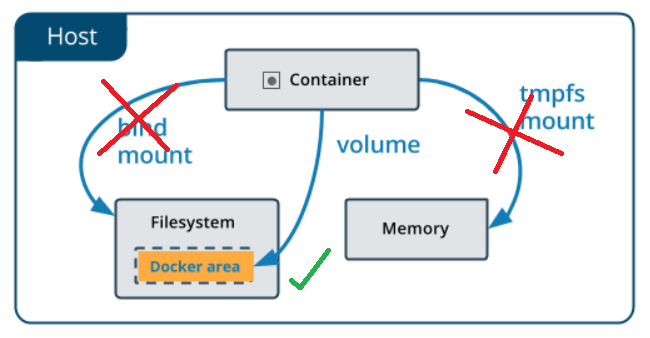
\includegraphics[width=0.75\textwidth]{figures/volumen.png}
    \caption{Volumen de Docker}
    \label{volumen}
\end{figure}

Se puede ver un volumen como una forma de almacenar datos persistentes en el sistema de ficheros local del cliente, necesario para gestionar el acceso al \textit{hardware} entre otras cosas para esta herramienta, que permanece completamente aislado de la funcionalidad central y el \textit{core} de la máquina anfitriona. Esto significa que el contenedor sólo podrá actuar sobre el contenido del volumen y no sobre el contenido externo, pero se podrá beneficiar de todas las ventajas que ofrece el administrador del sistema de archivos del sistema operativo del usuario. Así, aún en el supuesto de que se tratase de utilizar la ``Ejecución Mixta'' en conjunto con una aplicación robótica maliciosa (supuesto muy improbable), el mayor daño posible que se podría causar se reduciría a parar y reiniciar el contenedor, eliminándose todo indicio de código maligno o sospechoso.

\subsubsection{Capa de Bajo Nivel}

La capa de menor nivel y mayor grado de restricción de la herramienta es la que hemos denominado Capa de Bajo Nivel, cuya puerta es sólo visible para el secuenciador del módulo de gestión.
\clearpage
\begin{figure}[!hbtp]  \centering\noindent
    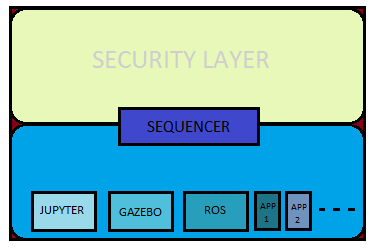
\includegraphics[width=0.6\textwidth]{figures/layer1.png}
    \caption{Módulo de Gestión: Capa de Gestión del Bajo Nivel}
    \label{layer1}
\end{figure}

Una vez resuelta la comunicación y superada la seguridad, el motor de la ``Ejecución Mixta'' debe decidir qué se necesita en todo momento según las peticiones que recibe, y más importante, a quién redirige cada mensaje. Para la Capa de Comunicación, todos los mensajes tienen el mismo destinatario, en función de la conexión HTTPS que se abre para comunicar el lado servidor y el cliente. Este receptor único es un módulo secuenciador, configurado y levantado a través de un \textit{entrypoint} que activará en cada momento la aplicación, herramienta o plataforma auxiliar que se necesite para satisfacer las peticiones de la aplicación robótica, y organizará el canal de bajo nivel para que no se produzcan colisiones durante el proceso. La forma de gestionar la secuenciación se basa en la apertura de nuevos sub-canales de comunicación, ya en un entorno puramente local o \textit{localhost}, y en una redirección de la información obtenida en cada sub-canal hacia el canal HTTPS principal, formateando cada paquete de información según su fuente, su destinatario en la aplicación robótica y su prioridad, a través de cabeceras y estructuras de datos JSON fácilmente procesables por una aplicación web, y accesibles a través del API público de la Capa de Aplicación (Figs. \ref{nb_put_req} y \ref{exec_req}).

\begin{lstlisting}[language=bash, caption=Ejemplo de la parte HTTP de los mensajes]
PUT /api/contents/descarga_bundle.png HTTP/1.1
Host: 127.0.0.1:8888
Connection: keep-alive
Content-Length: 25899
Sec-Fetch-Mode: cors
Origin: http://localhost:8000
User-Agent: Mozilla/5.0 (X11; Linux x86_64) AppleWebKit/537.36
(KHTML, like Gecko) Chrome/77.0.3865.120 Safari/537.36
Content-Type: application/json
Accept: */*
Sec-Fetch-Site: cross-site
Referer: http://localhost:8000/local
Accept-Encoding: gzip, deflate, br
Accept-Language: es-ES,es;q=0.9
\end{lstlisting}

\begin{figure}[!hbtp]  \centering\noindent
    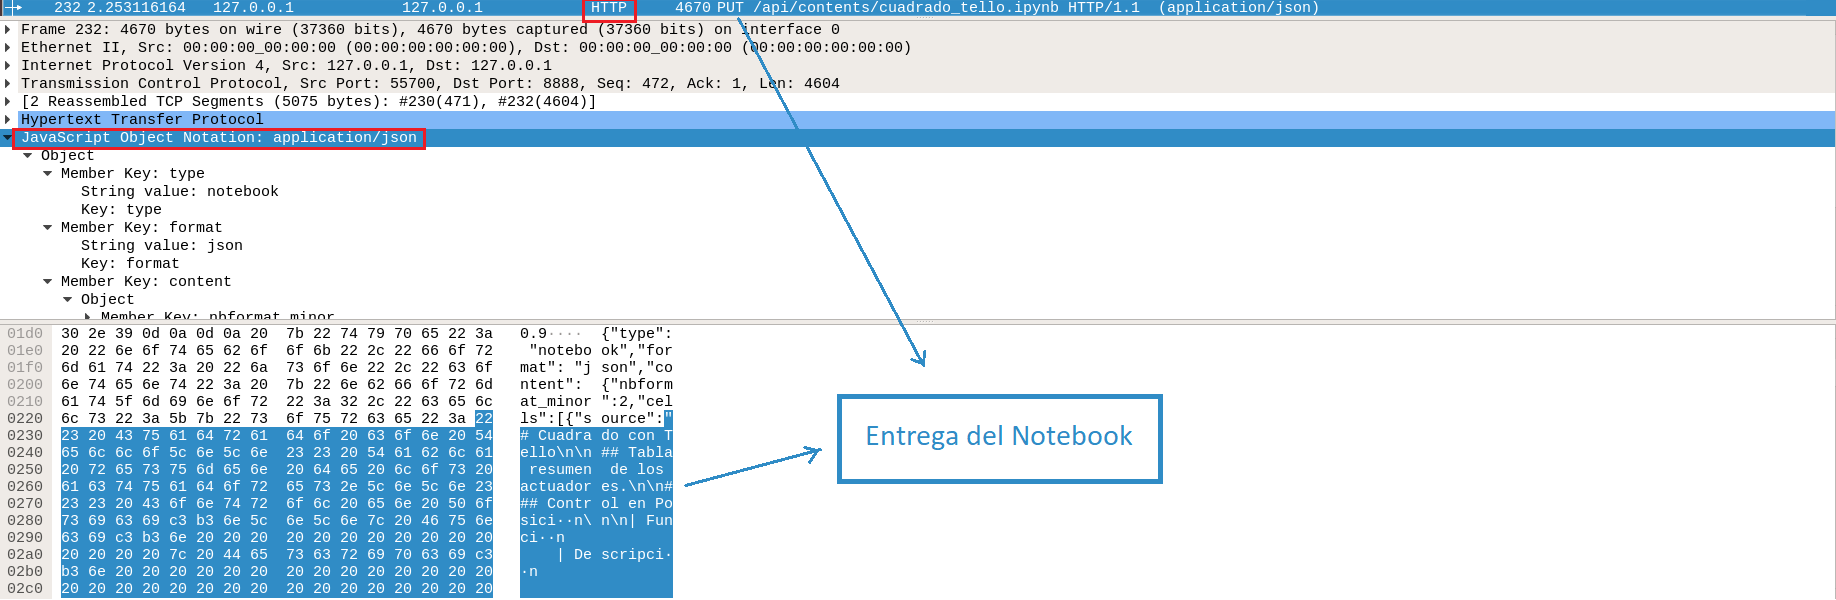
\includegraphics[width=1.05\textwidth]{figures/notebook_put_request.png}
    \caption{Mensaje de Entrega del Cuadernillo o Notebook}
    \label{nb_put_req}
\end{figure}

\begin{figure}[!hbtp]  \centering\noindent
    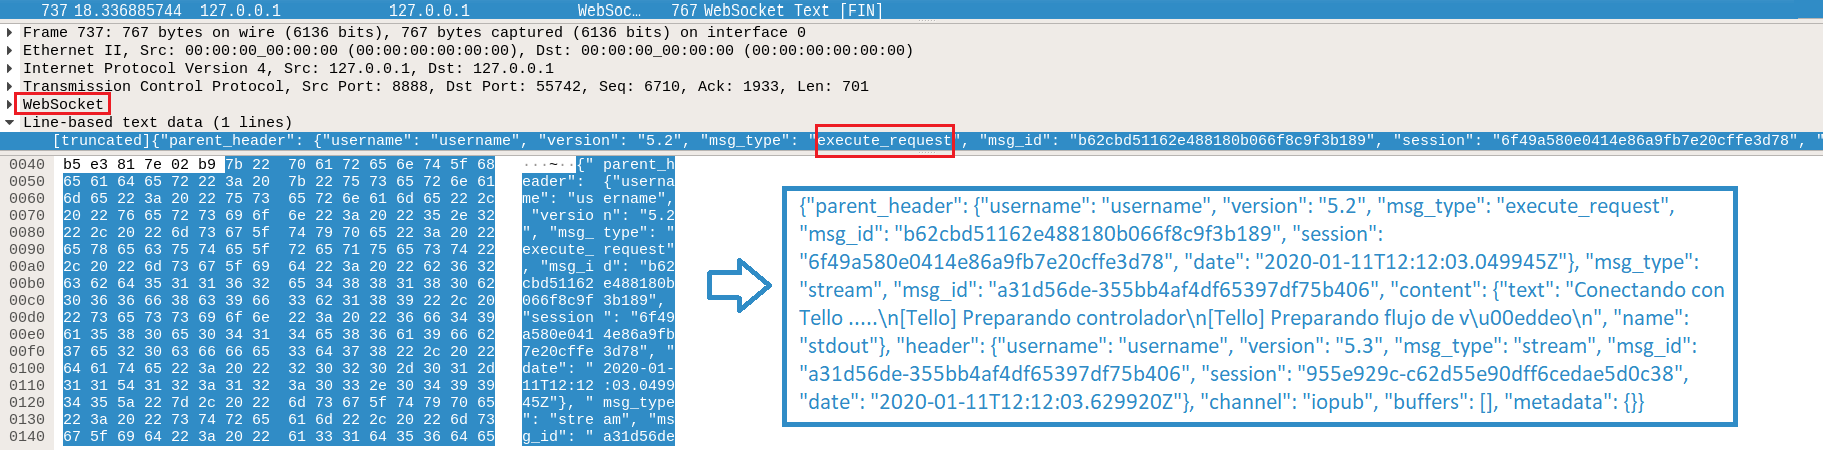
\includegraphics[width=1.05\textwidth]{figures/execute_request.png}
    \caption{Mensaje de Respuesta de Petición de Ejecución }
    \label{exec_req}
\end{figure}

Además, los diferentes programas que ejecutan en el interior del contenedor Docker en el servidor de ``Ejecución mixta'' necesitan un mecanismo de intercomunicación de tipo p2p, sin pasar por todo el mecanismo de transmisión, recepción y procesado descrito anteriormente como parte de la arquitectura, para facilitar la colaboración entre ellos sin sucumbir a problemas de tipo \textit{jitter}, grandes retardos de extremo a extremo o pérdidas de información y largas esperas de reenvios que caracterizan a muchos enlaces de Internet basados en TCP/IP. Para implementar este mecanismo de comunicación interna aprovecharemos las herramientas de ROS, donde el secuenciador tendrá el rol de \textit{MASTER} y las diferentes plataformas y aplicaciones en ejecución actuarán como suscriptores y publicadores de información a través de \textit{topics} conocidos por todos. Así, se dispondrá por ejemplo un HAL API (\textit{Hardware Abstraction Layer}) que permitirá a todos los programas que lo requieran el acceso a las interfaces de sensado y actuación del robot, ya sea real (con \textit{plugins} y \textit{drivers} reales involucrados) o simulado (con \textit{drivers} virtuales). Este método de intercomunicación facilita el crecimiento de la red de agentes (que simplemente ``escuchan'' la información del canal que les conviene y publican los datos que generan que pueden resultar útiles para otros procesos) que se puede lanzar para proporcionar mayor volumen de información a la aplicación robótica remota, y por tanto a la construcción de aplicaciones remotas más ricas que no produzcan carga computacional en el lado servidor de la misma gracias a la ``Ejecución Mixta''.

\section{Funcionamiento}
\subsection{Flujograma}

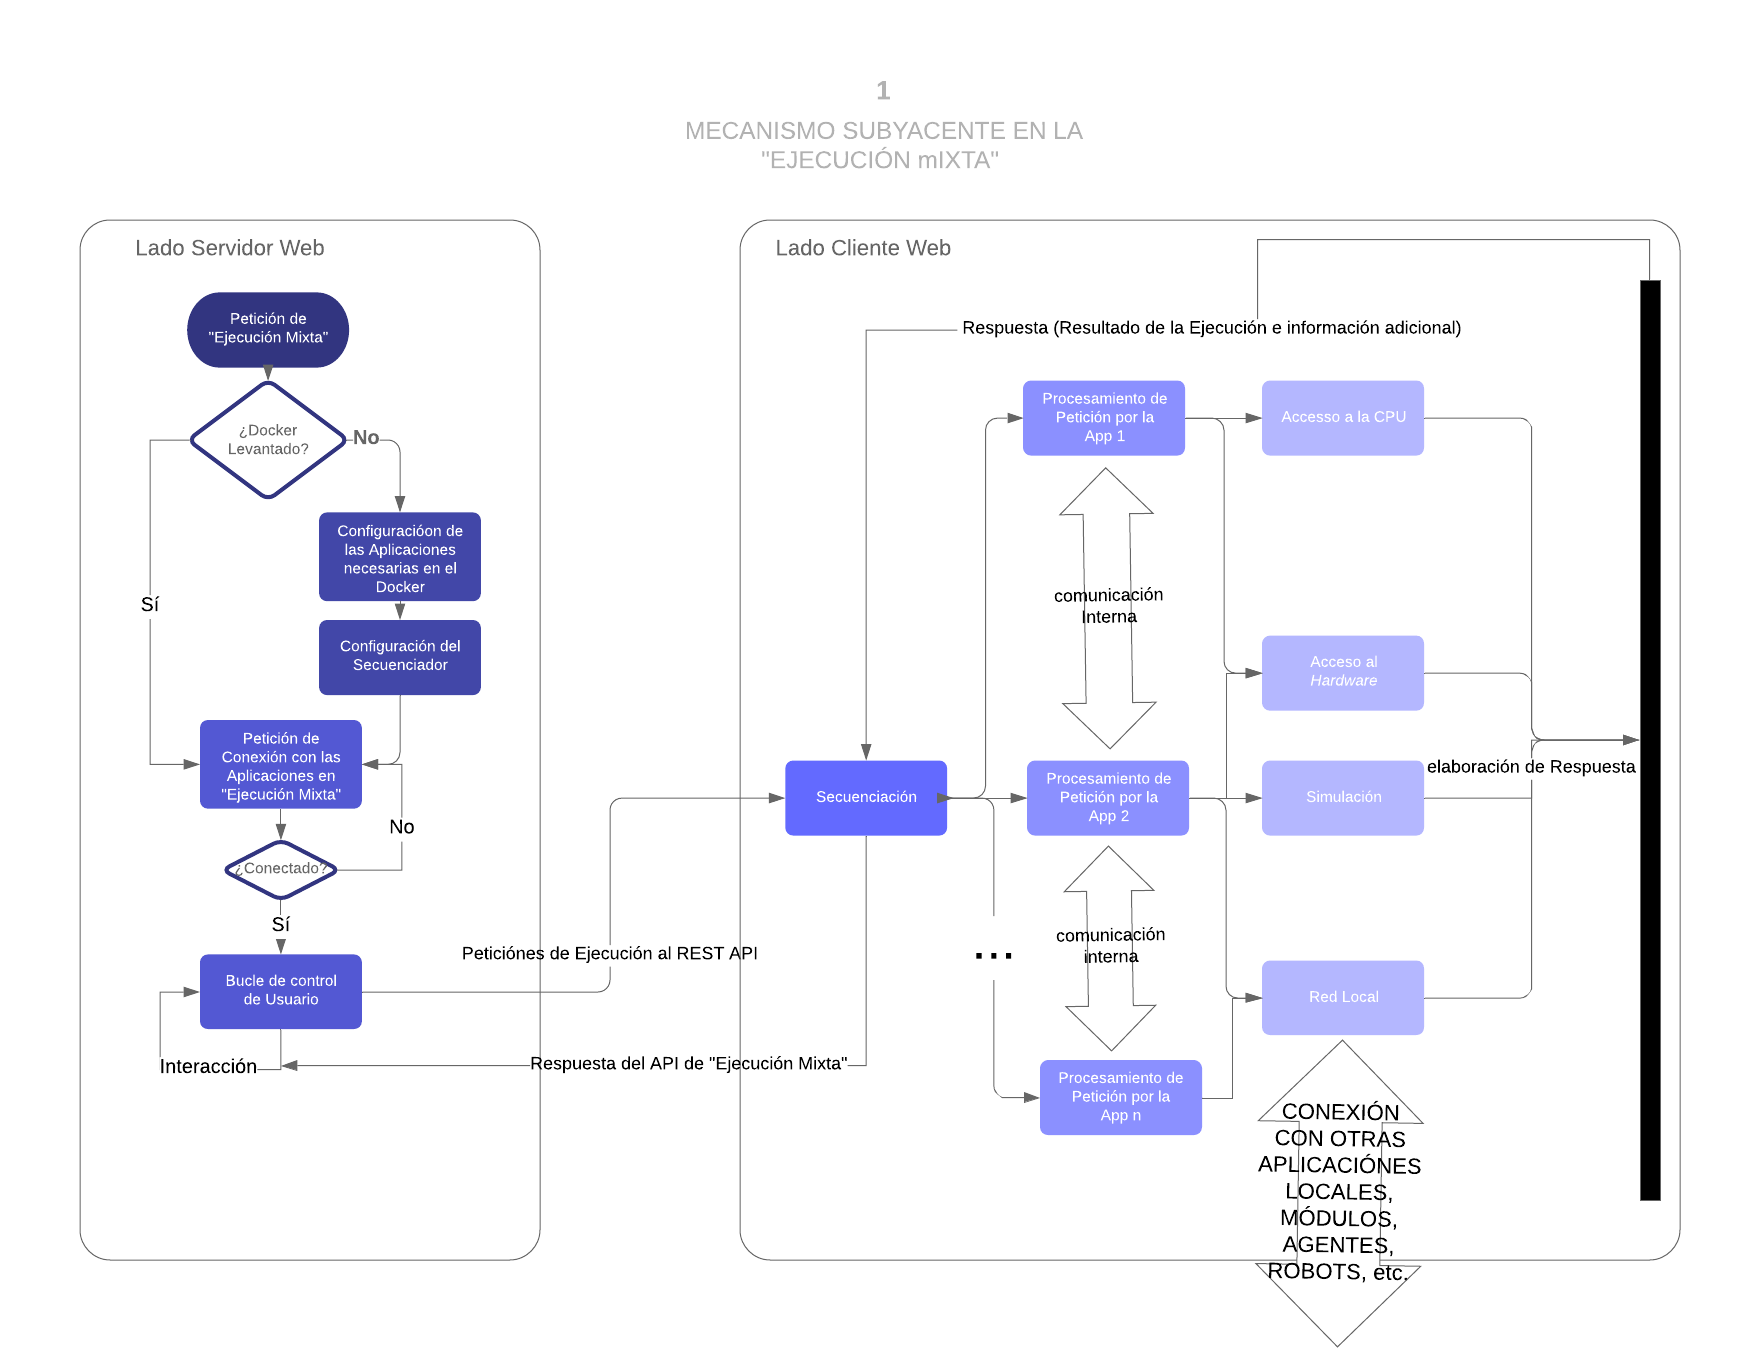
\includepdf[addtolist={1,figure,{Flujograma},flowchart}]{figures/flowchart.png}

\subsection{Ejecución Mixta: Diagrama de flujo}

Para explicar el mecanismo que desata el uso de la ``Ejecución Mixta'' por parte de una aplicación, se utilizará el caso hipotético de un usuario que dispone de un robot móvil con conectividad inalámbrica a través de una red propia con visibilidad a la red local del usuario, al ser la del robot una subred de ésta.

Apoyándonos en el diagrama de flujo anterior (Fig. \ref{flowchart}), el proceso comienza con la realización de la petición inicial de ``Ejecución Mixta'', que se corresponde con la solicitud hecha por el usuario a la aplicación remota de un servicio que utiliza senda herramienta de ejecución. Dado que la aplicación web remota es la que ofrece el servicio solicitado, es también la aplicación la que conoce la configuración de ``Ejecución Mixta'' necesaria para el proceso, así como la combinación de aplicaciones de las que va a requerir información durante la ejecución que deben iniciarse en el lado cliente web. Es entonces cuando se envía esta configuración al cliente, quien debe iniciar el contenedor Docker que aloja la herramienta. Una vez iniciado, se ha de conectar con cada una de las aplicaciones contenidas en la herramienta de ejecución desde la aplicación web. Como se mencionó con anterioridad, esto desencadena en el servidor web una petición inicial al API de ``Ejecución Mixta'', que pasa a desempeñar el rol de cliente de ``Ejecución Mixta'', y que hace una solicitud de conexión. Si los mecanismos de seguridad se resuelven con éxito, el secuenciador del lado cliente web, que actúa como servidor de ``Ejecución Mixta'', garantiza el acceso de la aplicación remota a la ejecución. Es entonces cuando se inicia el servicio que el cliente web solicitó en primera instancia, ingresando en un bucle de control y eventos de la misma forma que sucedería en cualquier otro tipo de aplicación web. En este bucle, la aplicación web atiende permanentemente las interacciones del usuario web, quien generará eventos en el contexto de la aplicación web, y que podrá generar peticiones concretas de ejecución local. Cuando se produce este tipo de petición es cuando la aplicación hace uso de la ``Ejecución Mixta'' para lanzar el código del usuario web, escrito y almacenado remotamente desde su punto de vista, sobre el \textit{hardware} local al usuario. Como se comentó, estas peticiones viajan con un formato concreto a modo de protocolo con destino al secuenciador de ``Ejecución Mixta'', quien ya en el entorno local es capaz de analizar la petición y redirigirla convenientemente a su destinatario o destinatarios. Los receptores finales de estas solicitudes serán las diferentes aplicaciones lanzadas para soportar el servicio web, que se especificaban en el \textit{entrypoint} de configuración inicial del secuenciador. Es entonces cuando los receptores pueden procesar la petición, siempre y cuando el método solicitado esté soportado por el REST API de ``Ejecución Mixta''. El receptor principal será siempre Jupyter, pues es quién tendrá la capacidad de ejecutar código sobre la CPU local o el robot. También habrá un volumen considerable de peticiones de simulación, con el fin de mantener siempre actualizado el estado de la simulación, si existe, en la aplicación web y su interfaz gráfico, que es el que ve el usuario. Para el caso planteado, incluso habrá peticiones concretas o resultados de la ejecución del código que desembocarán en el establecimiento de un nuevo canal de comunicación a través de la red del cliente web. Como se puede ver en el diagrama anterior, este canal se puede utilizar para conectar el resultado de la ``Ejecución Mixta'' a cualquier otra aplicación externa del lado servidor de ejecución preparada para recibir los mensajes de respuesta que se generan. Esto hace crecer la potencia y el alcance de la ejecución, y las posibilidades de servicio web que se puede ofrecer. En el caso del ejemplo, la ejecución generaría mensajes que deben ser enviados al receptor del robot móvil a través de la red inalámbrica, que se materializarían en la actualización de sus actuadores y sensores. Según sea el mensaje, el robot devolverá cierta información. Con esta información, y la proveniente del resultado del procesamiento de la petición entrante por cada aplicación receptora, se compone un único mensaje de respuesta que se reenvía a través del API al servidor web, con toda la información que el servicio espera para su correcto funcionamiento. El ejemplo para este caso pueden ser mensajes de éxito o fracaso de acceso a las interfaces del robot y el resultado concreto de la ejecución solicitada. La información se usa en última instancia para actualizar el interfaz y el estado del servicio para que el cliente web pueda ver el resultado de su interacción. Se finalizaría así la iteración del proceso de ``Ejecución Mixta'' y quedaría a la espera de nuevas peticiones hasta la solicitud de finalización de ejecución, con la cual se liberaría la memoria asignada a todos los procesos en el lado servidor de ejecución y se detendría el contenedor de forma segura, pudiéndose dar por terminado el servicio web.